\documentclass[12pt]{article}
\usepackage{amsmath,amsfonts,amssymb}
\usepackage{graphicx}
\usepackage{hyperref}
\usepackage{authblk}
\usepackage[backend=biber]{biblatex}
\addbibresource{../references.bib}
\title{Observer-Centric Bitstring Universes: A Minimal Informational Model of Reality}
\author{Juha Meskanen}
\date{July 2025}

\begin{document}

\maketitle

\begin{abstract}
    We present a discrete, observer-based model of the universe grounded in bitstring information theory. In this minimal setting, we define observers as sequences of finite bitstrings and investigate their persistence within possible universes composed of frames of bits. The model introduces a similarity metric for observer survival, proposes an entanglement-like phenomenon via shared memory fragments, and reinterprets the wavefunction as a compressed extrapolation over observer trajectories. This framework challenges traditional physical ontology, suggesting that reality is observer-centric and informational at its core.

\end{abstract}


\section*{Relation to Previous Work}

In prior papers, we developed the foundations of an informational ontology of physics:

\begin{itemize}
    \item \textbf{Paper 1} introduced the idea that human observers are formal axiomatic systems defined by DNA and that time and pain emerge from internal informational transitions.
    \item \textbf{Paper 2} demonstrated that real-world physical systems (e.g., black holes) and computational simulations are informationally equivalent, interpreting the black hole singularity as a zero-entropy trace.
    \item \textbf{Paper 3} explored the time-reversed case: a zero-entropy state giving rise to emergent structure as entropy increases, modeled via simple bitstring simulations.
\end{itemize}

This fourth paper closes the loop by showing how quantum-like behavior—interference, entanglement, and wavefunction evolution—emerges naturally within the same observer-centric, information-theoretic framework.

We explore a radically minimalist foundation for physics based on bitstrings and observer-centric reasoning. In this model, the universe is not something that evolves over time according to dynamical rules, but rather a collection of static information patterns in which observers find themselves embedded. Thus, what we call \emph{reality} is the subset of bitstring universes that contain coherent observer trajectories.


\section{Observational Assumptions}

In order to model a minimal universe we assume four observational assumptions. These are not metaphysical claims, but empirically grounded regularities, each supported by real-world examples or established computational models. They are deliberately minimal and falsifiable. If any one of them were shown to be invalid, the conclusions of this theory would not follow.

\paragraph{Assumption 1: Memory Requires Information Preservation}

\emph{Any observer capable of memory must preserve information across internal states.}

\vspace{0.2em}
This reflects the basic fact that for an observer to retain and recall experiences, the observer's internal structure must persist and encode past information. This is true of human cognition, digital memory systems, and even simple biological organisms.

\emph{Implication:} There must exist a substrate—physical or virtual—that allows for stateful information retention across time.

---

\paragraph{Assumption 2: Information Can Be Represented by Bitstrings}

\emph{Any physical or cognitive state can be encoded as a finite sequence of discrete symbols (e.g., a bitstring).}

\vspace{0.2em}
This is not a commitment to digital physics, but an acknowledgment that, for the purposes of modeling and communication, all observable phenomena can be encoded discretely. DNA, brain states, and digital computers all support this view.

\emph{Implication:} For modeling purposes, we can assume a discrete representation of observers and systems without loss of generality.

---

\paragraph{Assumption 3: Computation Is a Physical Process}

\emph{All physically realizable processes can be modeled as computation.}

\vspace{0.2em}
This aligns with the Church–Turing–Deutsch thesis and is broadly supported by the success of computational models in physics and biology. This assumption is empirical: no known physical process has been shown to lie outside computational modeling.

\emph{Implication:} Any observer or system can be described as a sequence of computational state transitions—an execution trace.

---

\paragraph{Assumption 4: Causality is Represented by Ordered States}

\emph{Causal structure corresponds to the sequential ordering of informational states.}

\vspace{0.2em}
In practice, we observe events as sequences: perception follows stimulus, memory encodes before retrieval, and measurements yield outputs after inputs. We assume that causality is experienced as an ordering of state transitions, not imposed externally.

\emph{Implication:} Time and causality are not primitive; they are emergent from the order in which informational states are experienced.

---

Together, these four assumptions provide the foundation for the theory that follows. They assert that memory, representation, computation, and causality are all observable features of physical reality. No metaphysical entities are required.

The remainder of this work shows that these assumptions—empirical, falsifiable, and widely supported—lead inevitably to the conclusion that the universe is fundamentally informational. All structure, from particles to consciousness, arises from the combinatorics of information patterns and their observer-relative interpretations.


\section{Framework and Definitions}

Let $B$ denote the total number of bits used to describe a universe. We define:

\begin{itemize}
    \item $\mathcal{U}_B$: the set of all possible universes composed of bitstrings of length $B$, partitioned into frames $f_i$ representing temporal slices.
    \item $O = \{o_1, o_2, \ldots, o_n\}$: a sequence of bitstrings representing the observer's memory and state across subjective time.
\end{itemize}

\subsection{Observer-Centric Universe Construction Principle (OCUCP)}


An observer exists in those universes $U \in \mathcal{U}_B$ where their memory patterns $o_i$ are statistically embedded within the universe frames $f_i$. The ontology is relational: observer existence is defined probabilistically by structural compatibility rather than by deterministic selection.


\subsection{Observer Contuinity Lemma (OCL)}

Let $O = \{o_1, o_2, \ldots, o_n\}$ be an observer trajectory, and $F = \{f_1, f_2, \ldots, f_n\}$ a candidate sequence of universe frames. Then, the observer can only \emph{remember} or \emph{experience} $F$ if:

\[
    \exists\ \epsilon > 0\ \text{ such that }\ \text{Similarity}(o_i, f_i) \ge \epsilon\ \text{ for all } i.
\]

In other words, the observer's internal structure must sufficiently overlap with the universe frames for continuity and memory to be possible. Memory is defined as structural self-similarity over time, not as causal flow.

\subsection{Similarity Metric and Observer Survival}

We define a similarity function $\text{Sim}(a, b)$ between two bitstrings. An observer $O$ survives a frame transition $o_i \to o_{i+1}$ only if $\text{Sim}(o_i, o_{i+1}) \ge \delta$ for some threshold $\delta$. This defines a selection criterion over possible trajectories.

\section{Compression and the Wavefunction}

We propose a new interpretation of the quantum wavefunction grounded in the logic of observer survival through compression.

\subsection{Compression Bias Principle (CBP)}

Let $C(F)$ denote the compressed length of a sequence of universe frames $F = \{f_1, \ldots, f_n\}$. Then, the number of observers that can embed within $F$ is inversely correlated with $C(F)$.

That is, smooth, regular, and compressible universes support more observers, simply because more observer trajectories can be accommodated within the same limited bit budget. Consequently, the universe we find ourselves in is likely to be highly compressible.

\subsection{Wavefunction as Compressed Continuation}

An observer’s internal model probabilistically extrapolates future frames by identifying structural regularities and compression patterns. This naturally leads to multiple possible continuations weighted by their compressibility, forming an informational “superposition” rather than a deterministic path.

\begin{itemize}
    \item The observer contains past states $\{o_1, \ldots, o_t\}$.
    \item It extrapolates possible futures $o_{t+1}, \ldots, o_{t+k}$ using pattern completion.
    \item If the compression basis is Fourier/sine-based (e.g., JPEG), extrapolation leads to smooth predictions.
    \item Multiple continuations are possible, forming a "superposition" within the observer's internal model.
\end{itemize}

Interference arises when extrapolated continuations reuse shared substrings. Thus, quantum phenomena emerge not from physical superposition, but from ambiguous extrapolations under compression logic. This model views the wavefunction as an efficient coding scheme, not as a physical entity.

\section{Entanglement and Shared Memory}

Entanglement is modeled as mutual constraint between observer subcomponents. If two observer bitstrings $A$ and $B$ share internal fragments and exist within a common universe $U$, then the observer can only survive in frames that preserve both. This shared structure constrains joint probabilities, introducing entanglement.

This is a structural, non-local correlation—not a causal interaction. It arises because the observer is a unified bitstring with branching substructures, not two separate agents.

\section{Simulation}

We present a simulation framework implementing the observer-centric model of universes. The simulation generates two-dimensional discrete spacetimes as sequences of bitstrings, representing the full ensemble of possible universe states. Observers do not actively select their continuations; instead, they find themselves statistically realized in those universe configurations that best sustain their continuations, e.g. match their memory patterns. Among the many consistent continuations, the observer's experience corresponds to the most probable or typical configurations as determined by structural similarity.

The simulation software implements the observer-centric model as follows:

\begin{itemize}
    \item \textbf{Bitstring Universe:} Generate all possible spacetime configurations as sequences of $n$-bit states over time.
    \item \textbf{Observers as Substrings:} Define an observer as a recurring bit pattern and use substring matching to detect compatible histories.
    \item \textbf{Similarity Score:} Score each universe path by how often the observer pattern appears, or by a more refined memory-similarity metric.
\end{itemize}

The program is hosted at:
\[
    \texttt{http://github.com/juham/simulations/paper4/observer\_centric\_universe.py}
\]

It takes the following input parameters:

\begin{itemize}
    \item Bit length $B$ of the universe.
    \item Number of frames $N$ to simulate, representing temporal evolution.
    \item List of observer bitstrings $O$, describing the evolution of observer memory and simpler particle bitstrings.
    \item Similarity threshold $\delta$ for observer survival.
\end{itemize}

The simulation generates a universe by randomly constructing frames of bits and then checks for observer compatibility. It tracks the evolution of observers across frames, visualizing their persistence and trajectories.

\begin{figure}[h!]
    \centering
    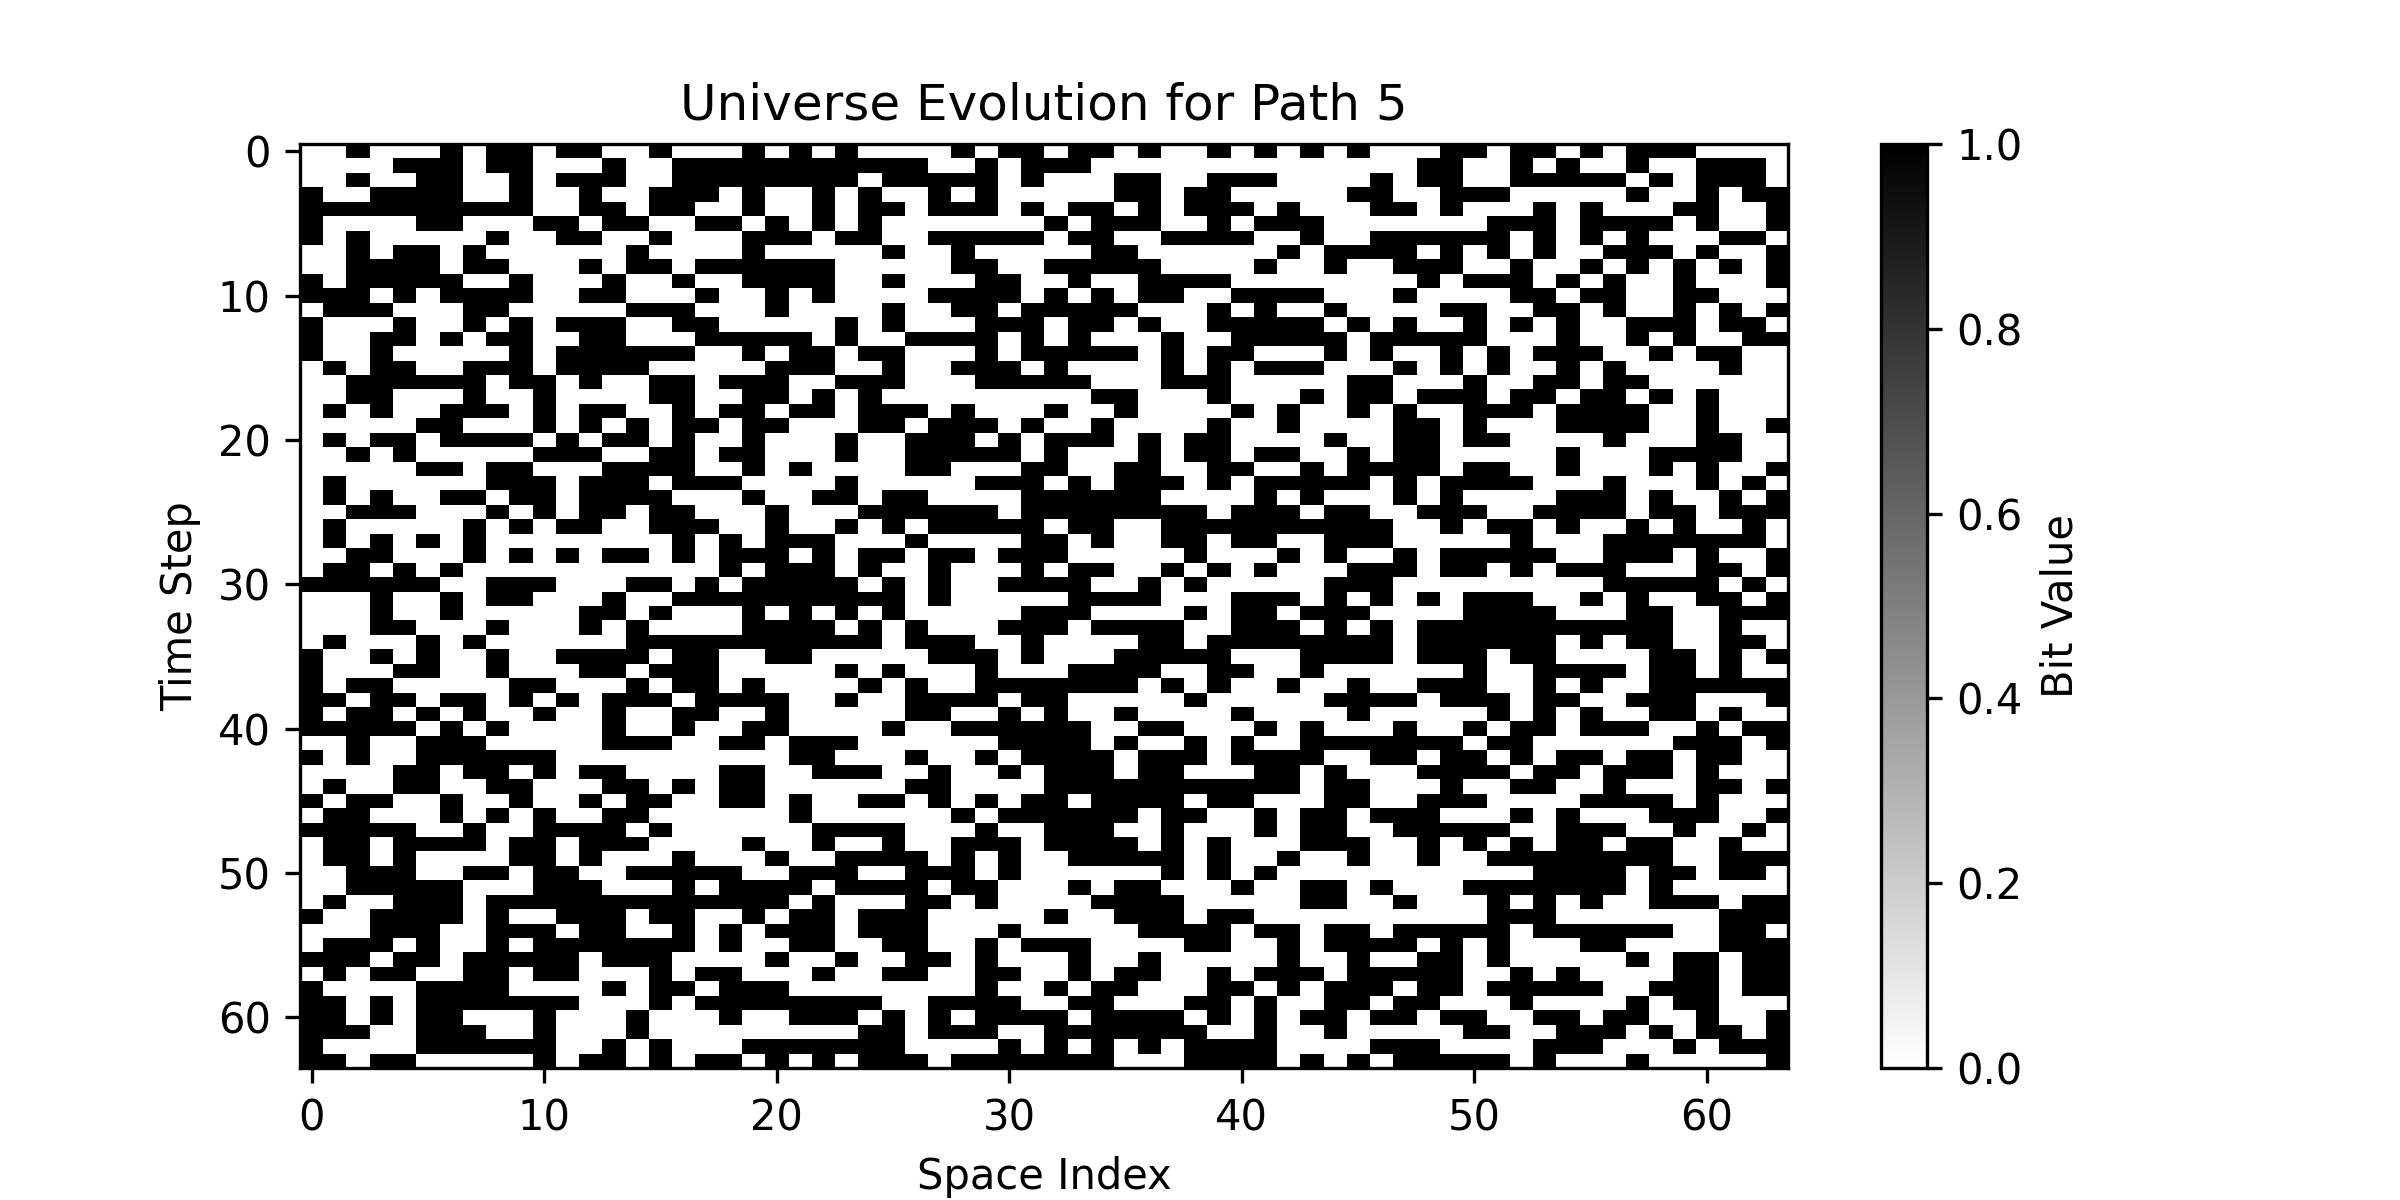
\includegraphics[width=1.0\textwidth]{figures/state_evolution_heatmap.png}
    \caption{State evolution of one of the simulated universes, including an observer. The evolution demonstrates coherence.}
    \label{fig:state_evolution}
\end{figure}

Particle trajectories are visualized as traces through the universe frames, showing how observers navigate the bitstring landscape. The simulation demonstrates that smooth trajectories can emerge when observers follow consistent patterns, even in a discrete universe.

\begin{figure}[h!]
    \centering
    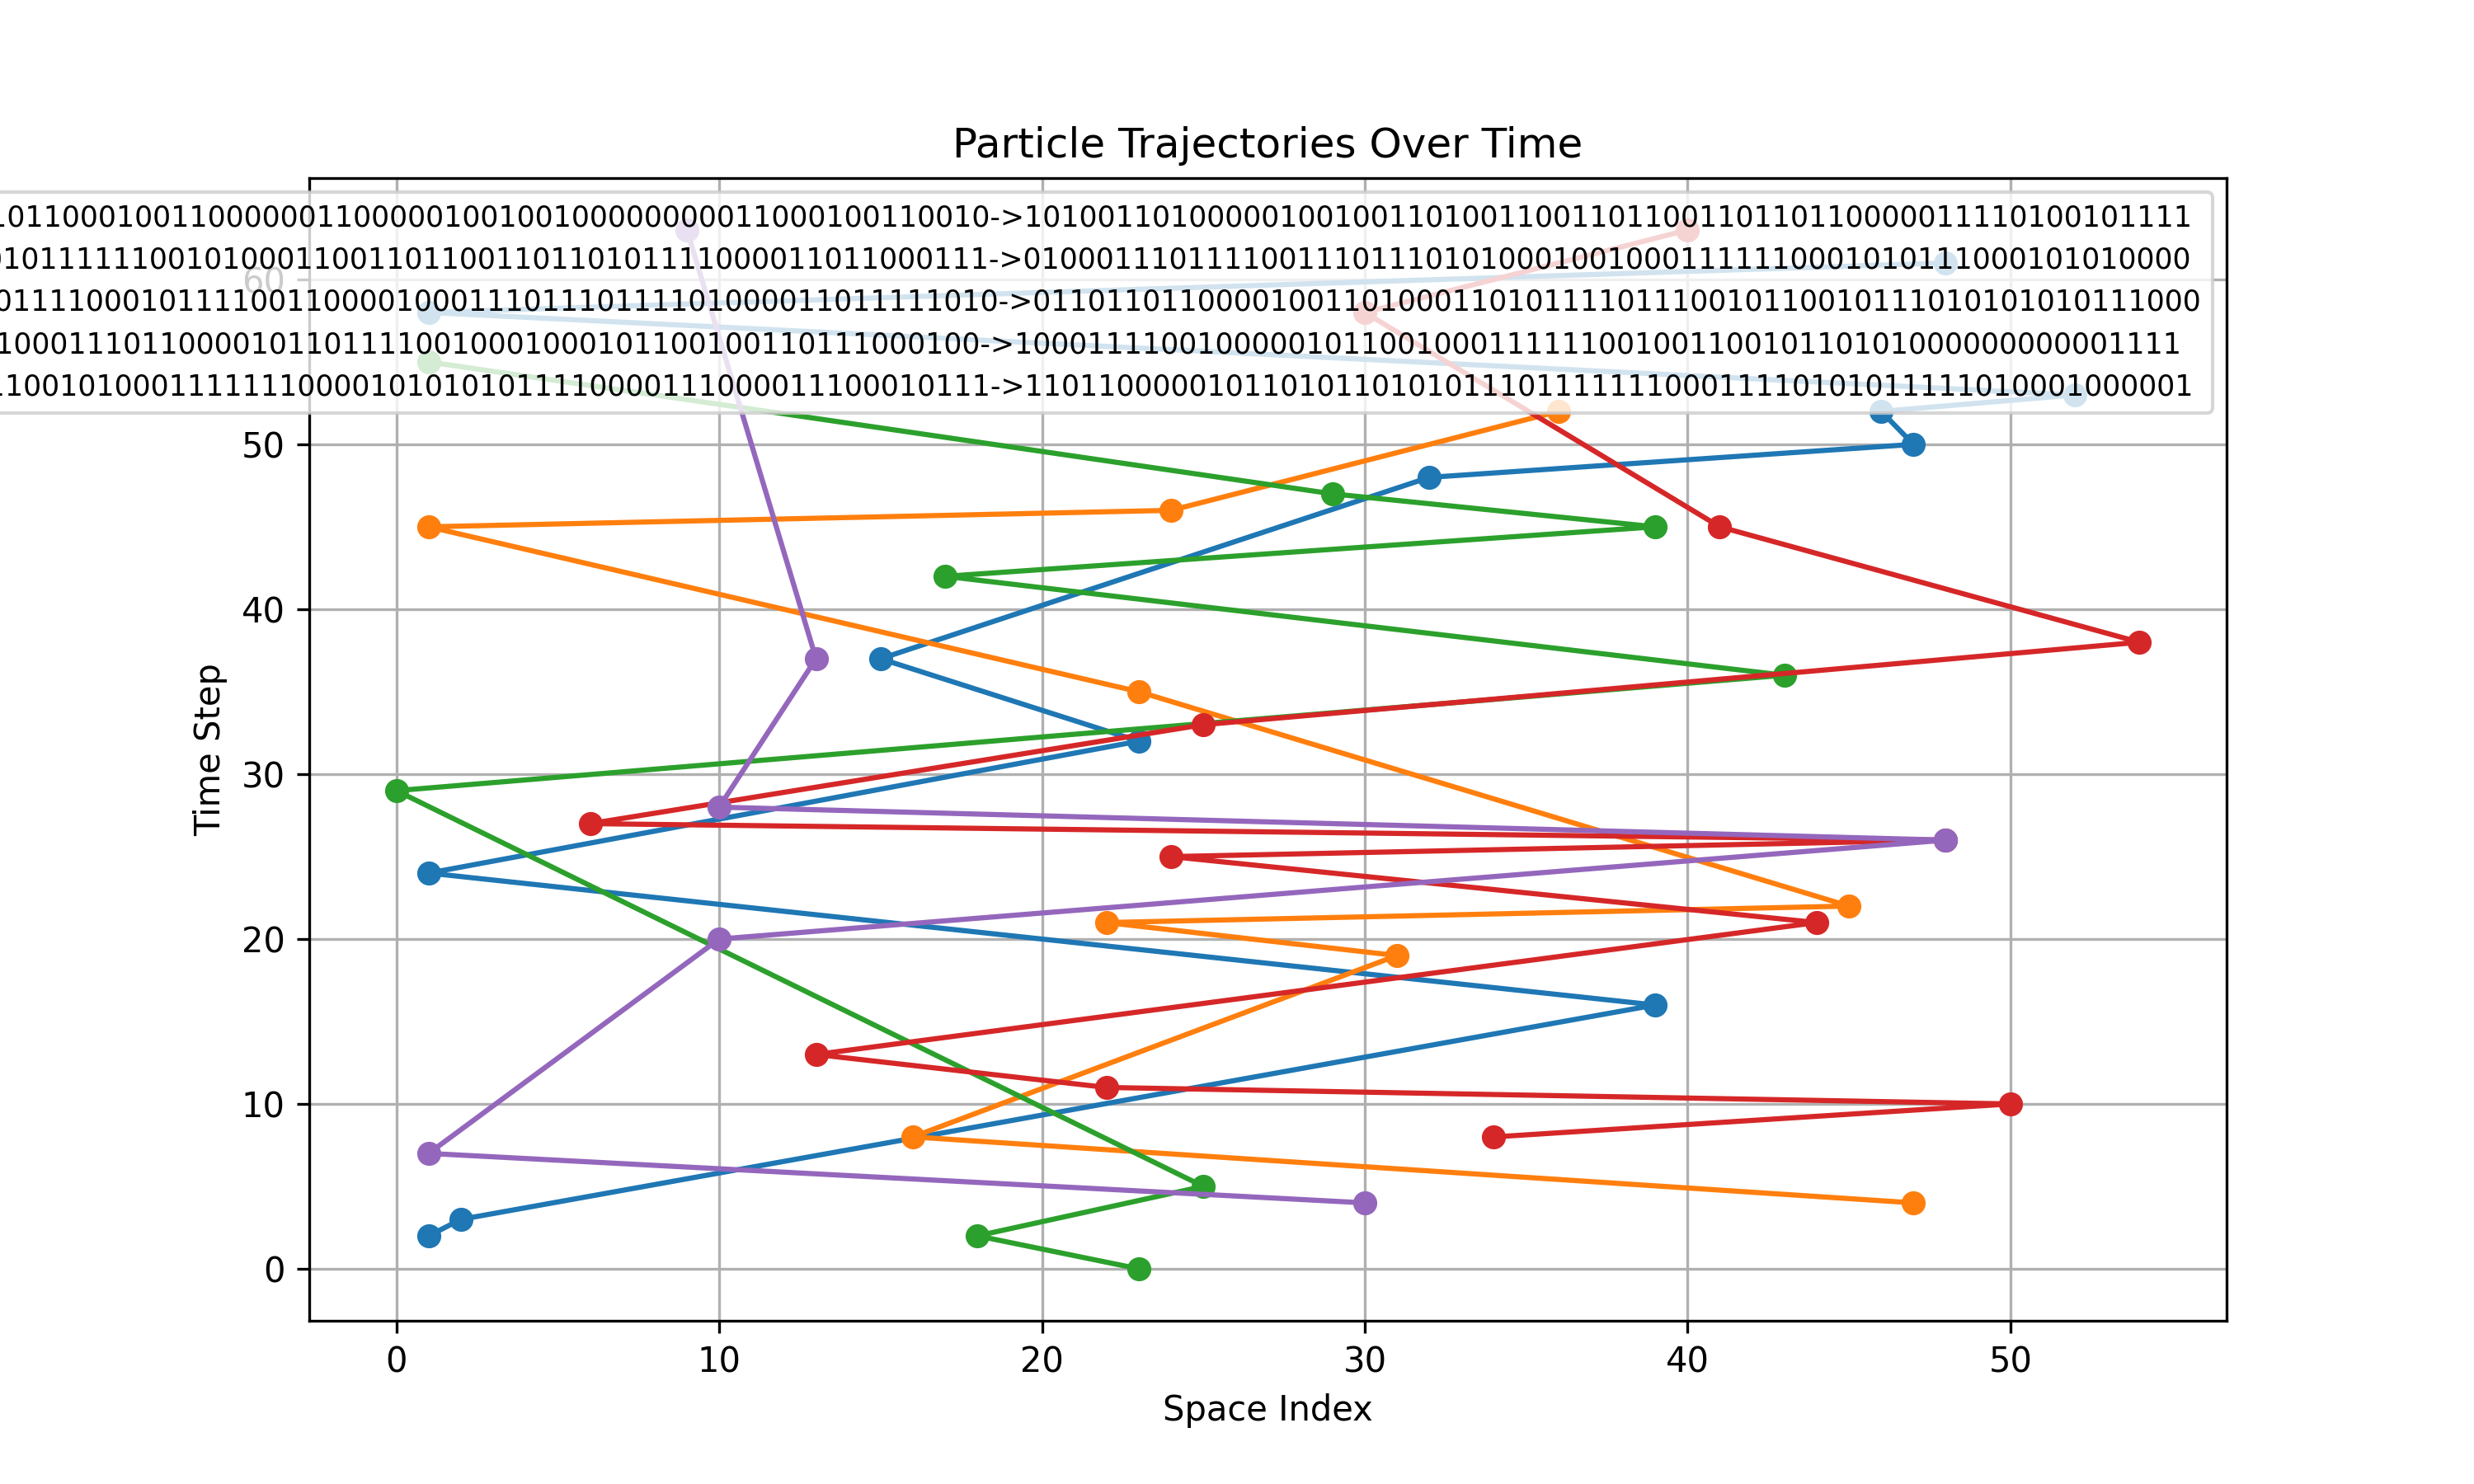
\includegraphics[width=1.0\textwidth]{figures/particle_trajectories.png}
    \caption{Particle traces showing that smooth trajectories emerge in universes that include coherent observer patterns.}
    \label{fig:particle_trajectories}
\end{figure}

A heatmap is generated to visualize the dynamics of the universe. Regions of high intensity indicate greater dynamical activity.

\begin{figure}[h!]
    \centering
    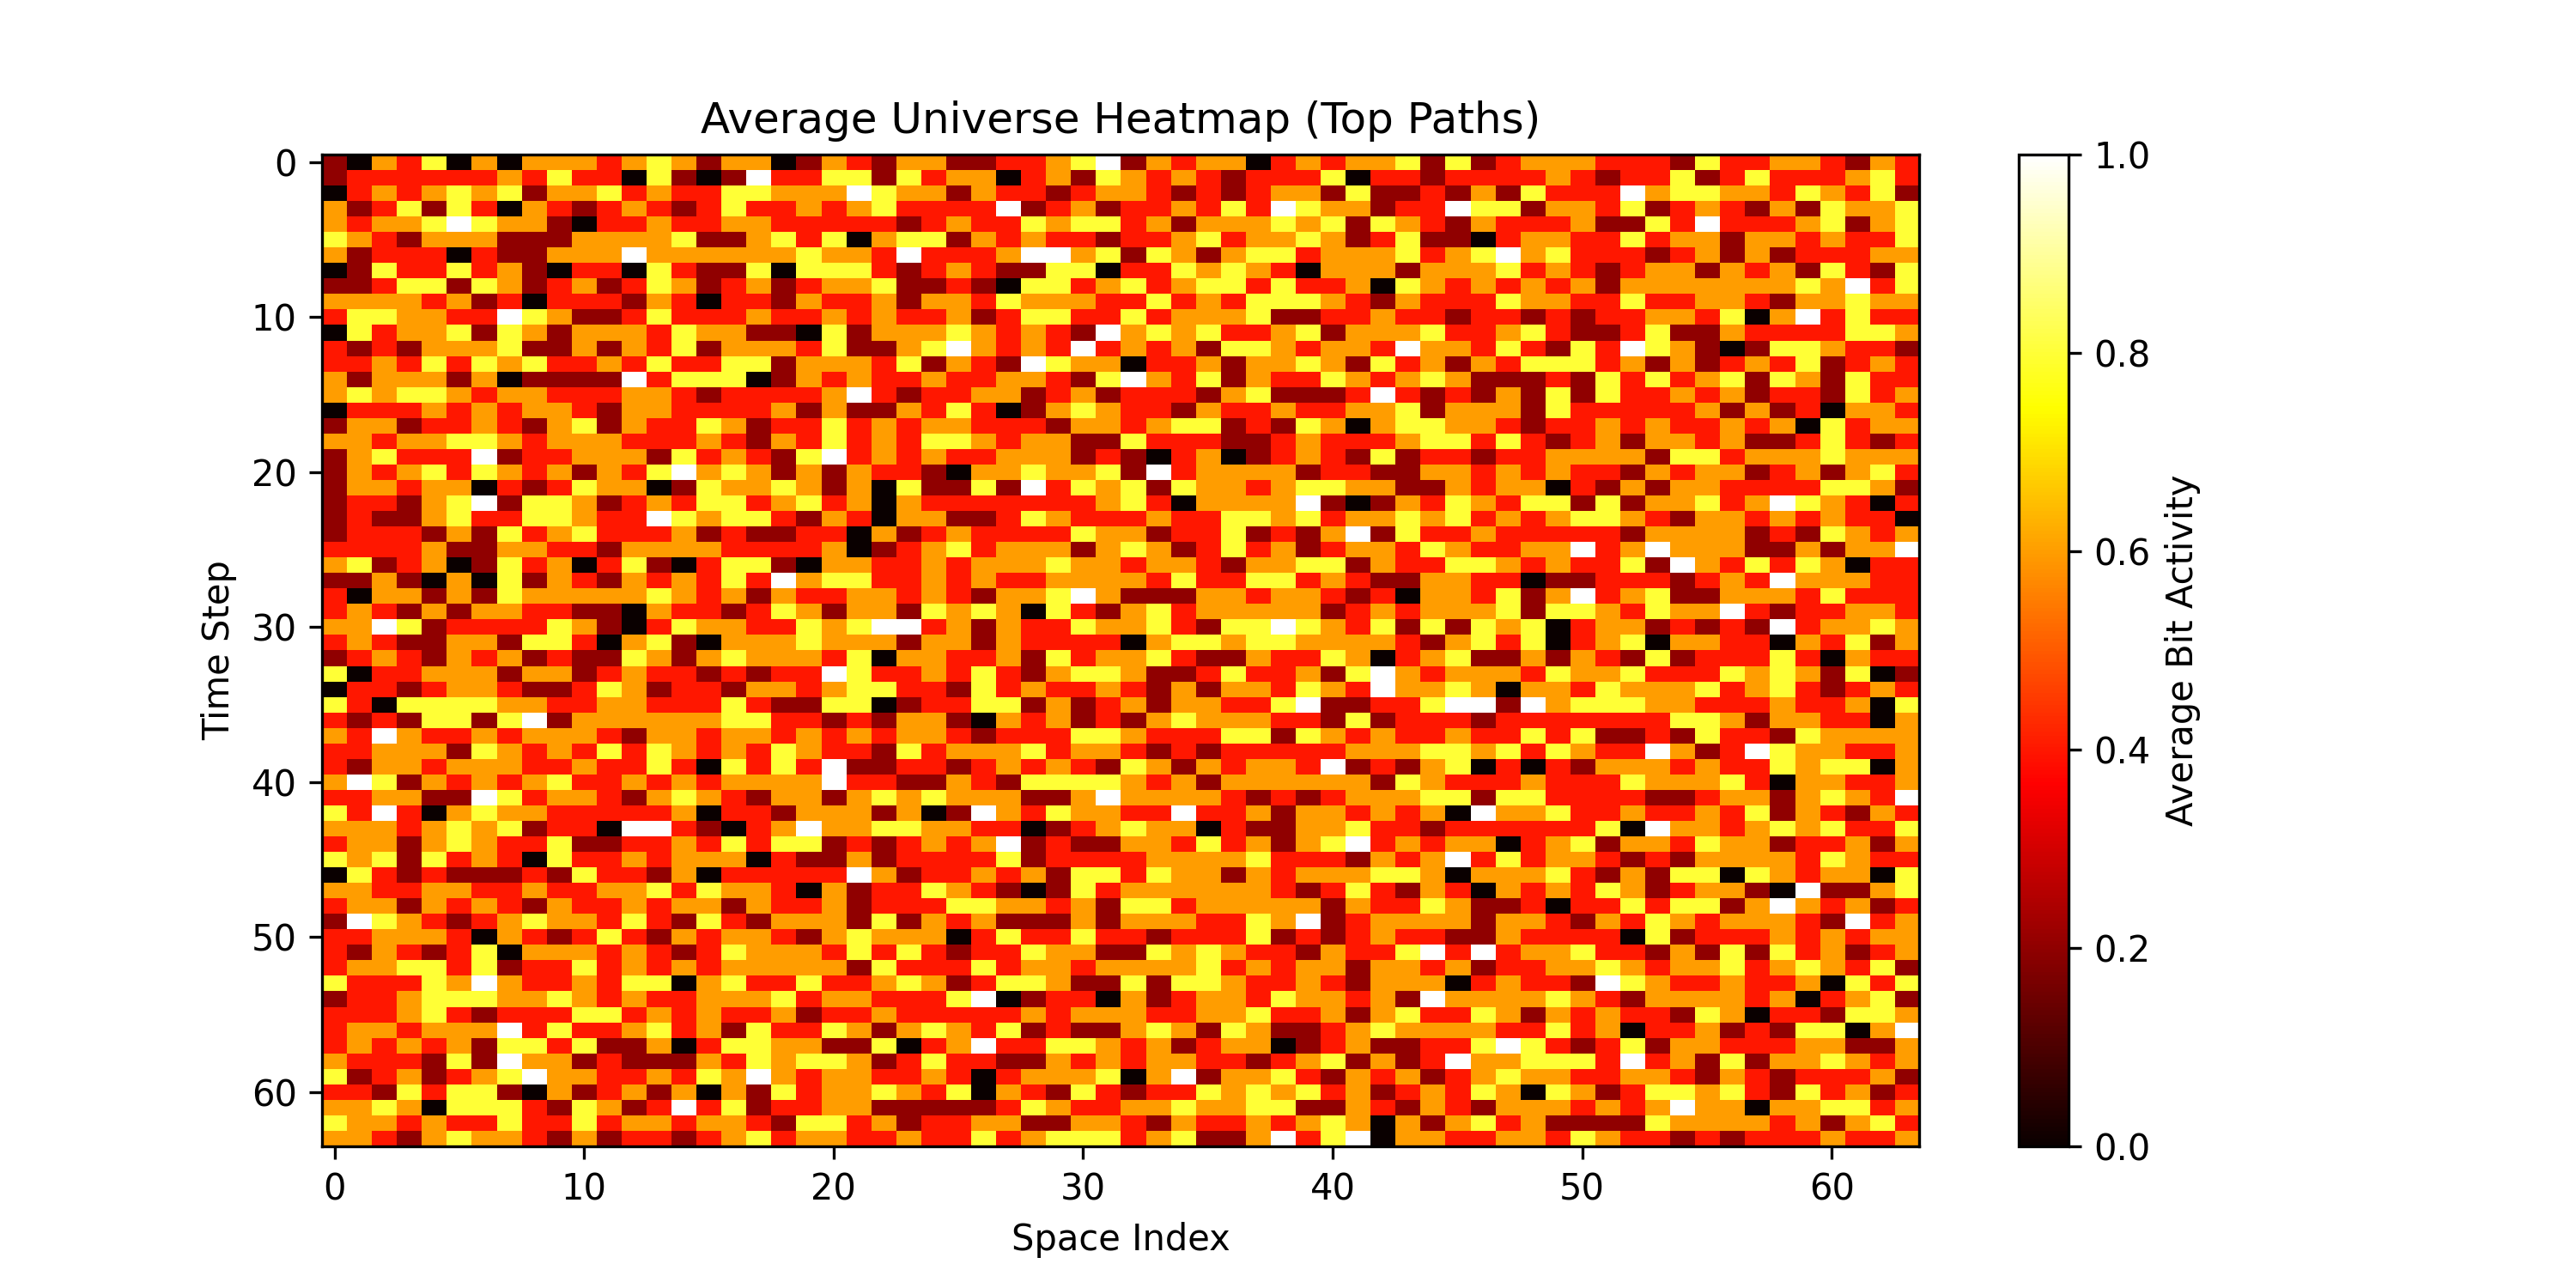
\includegraphics[width=1.0\textwidth]{figures/average_universe_heatmap.png}
    \caption{Heatmap visualizing the dynamics of the universe. Areas with a low density of particle trajectories indicate stable regions that change little over time. These worldlines are where observers or particles find consistent continuations.}
    \label{fig:average_universe_heatmap}
\end{figure}

\subsection{Wavefunction and Interference}

Why do we observe wave-like behavior in quantum mechanics? The wavefunction arises from the need to compress data. As the simplest periodic function, the sine wave offers an efficient basis for extrapolation. Observers prefer universe paths that align well with such wavefunctions, since those paths require fewer bits to describe. Universes with such structure are more probable because they support a greater number of embedded observers.

Interference emerges naturally when multiple such sine waves are superposed. Some paths reinforce alignment; others cancel. This mimics the Born rule of quantum mechanics: high amplitude corresponds to high probability, while destructive interference results in observer-incompatible paths.

\begin{figure}[h!]
    \centering
    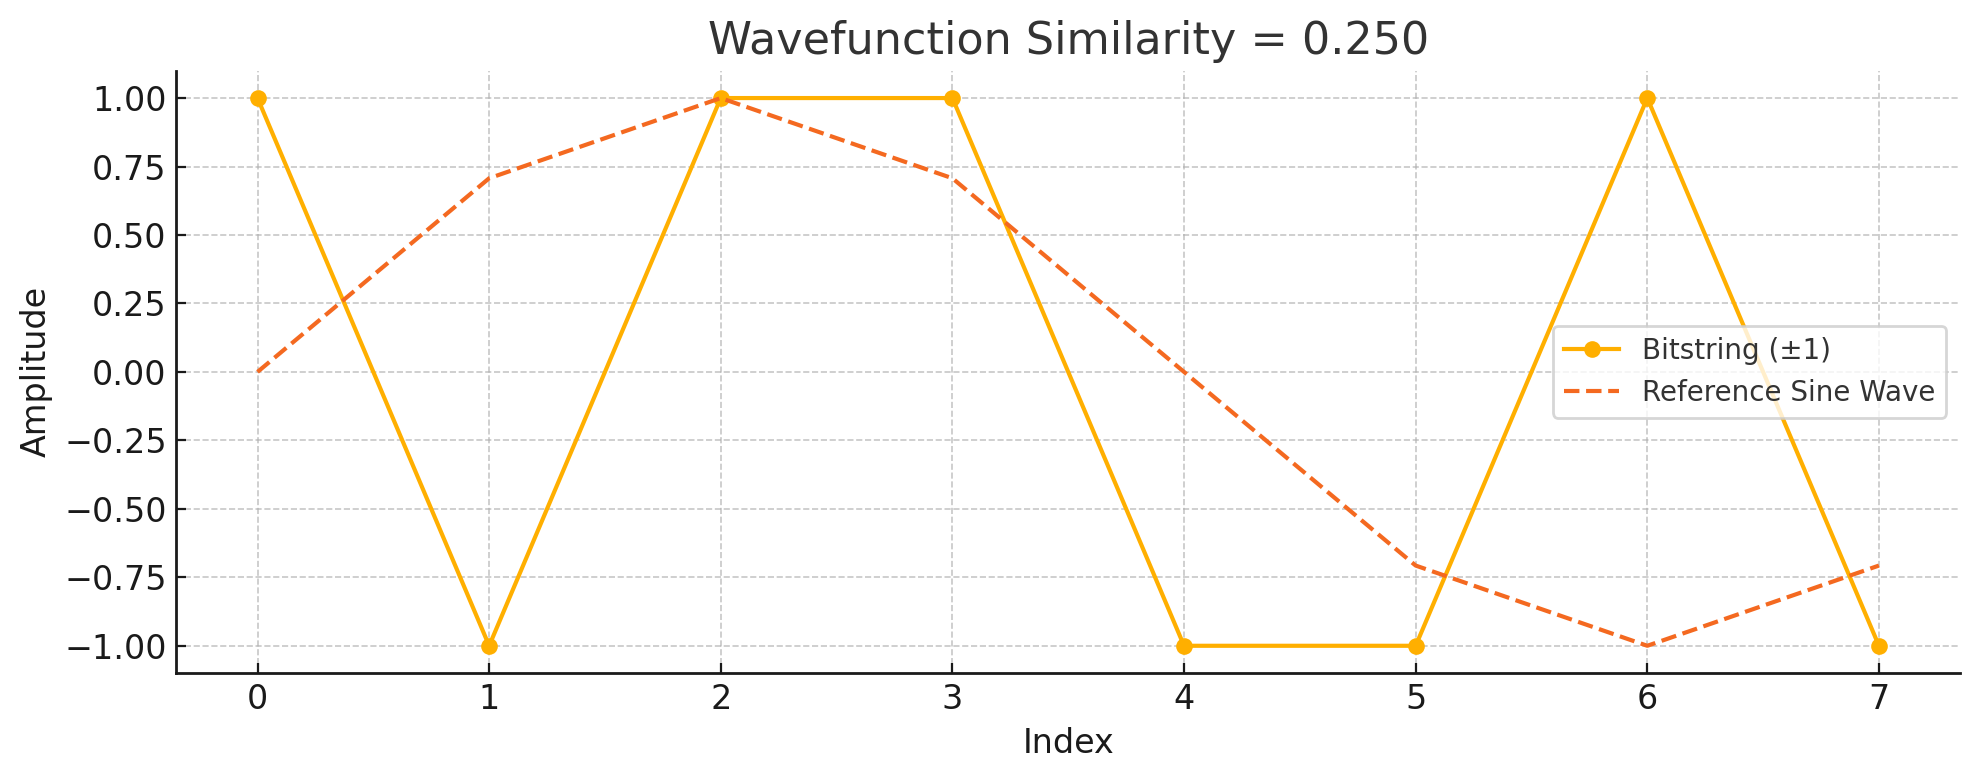
\includegraphics[width=1.0\textwidth]{figures/wavefunction_similarity.png}
    \caption{The chart shows how a bitstring (converted to ±1 amplitudes) aligns with a reference sine wave.
        The wavefunction similarity is calculated as the normalized dot product between these two curves.}
    \label{fig:wavefunction_similarity}
\end{figure}


This framework lets us interpret similarity as interference amplitude: when it's high, the observer's pattern resonates with a compressible (wave-like) universe. This links bit-level structure to emergent wavefunction behavior.

\begin{figure}[h!]
    \centering
    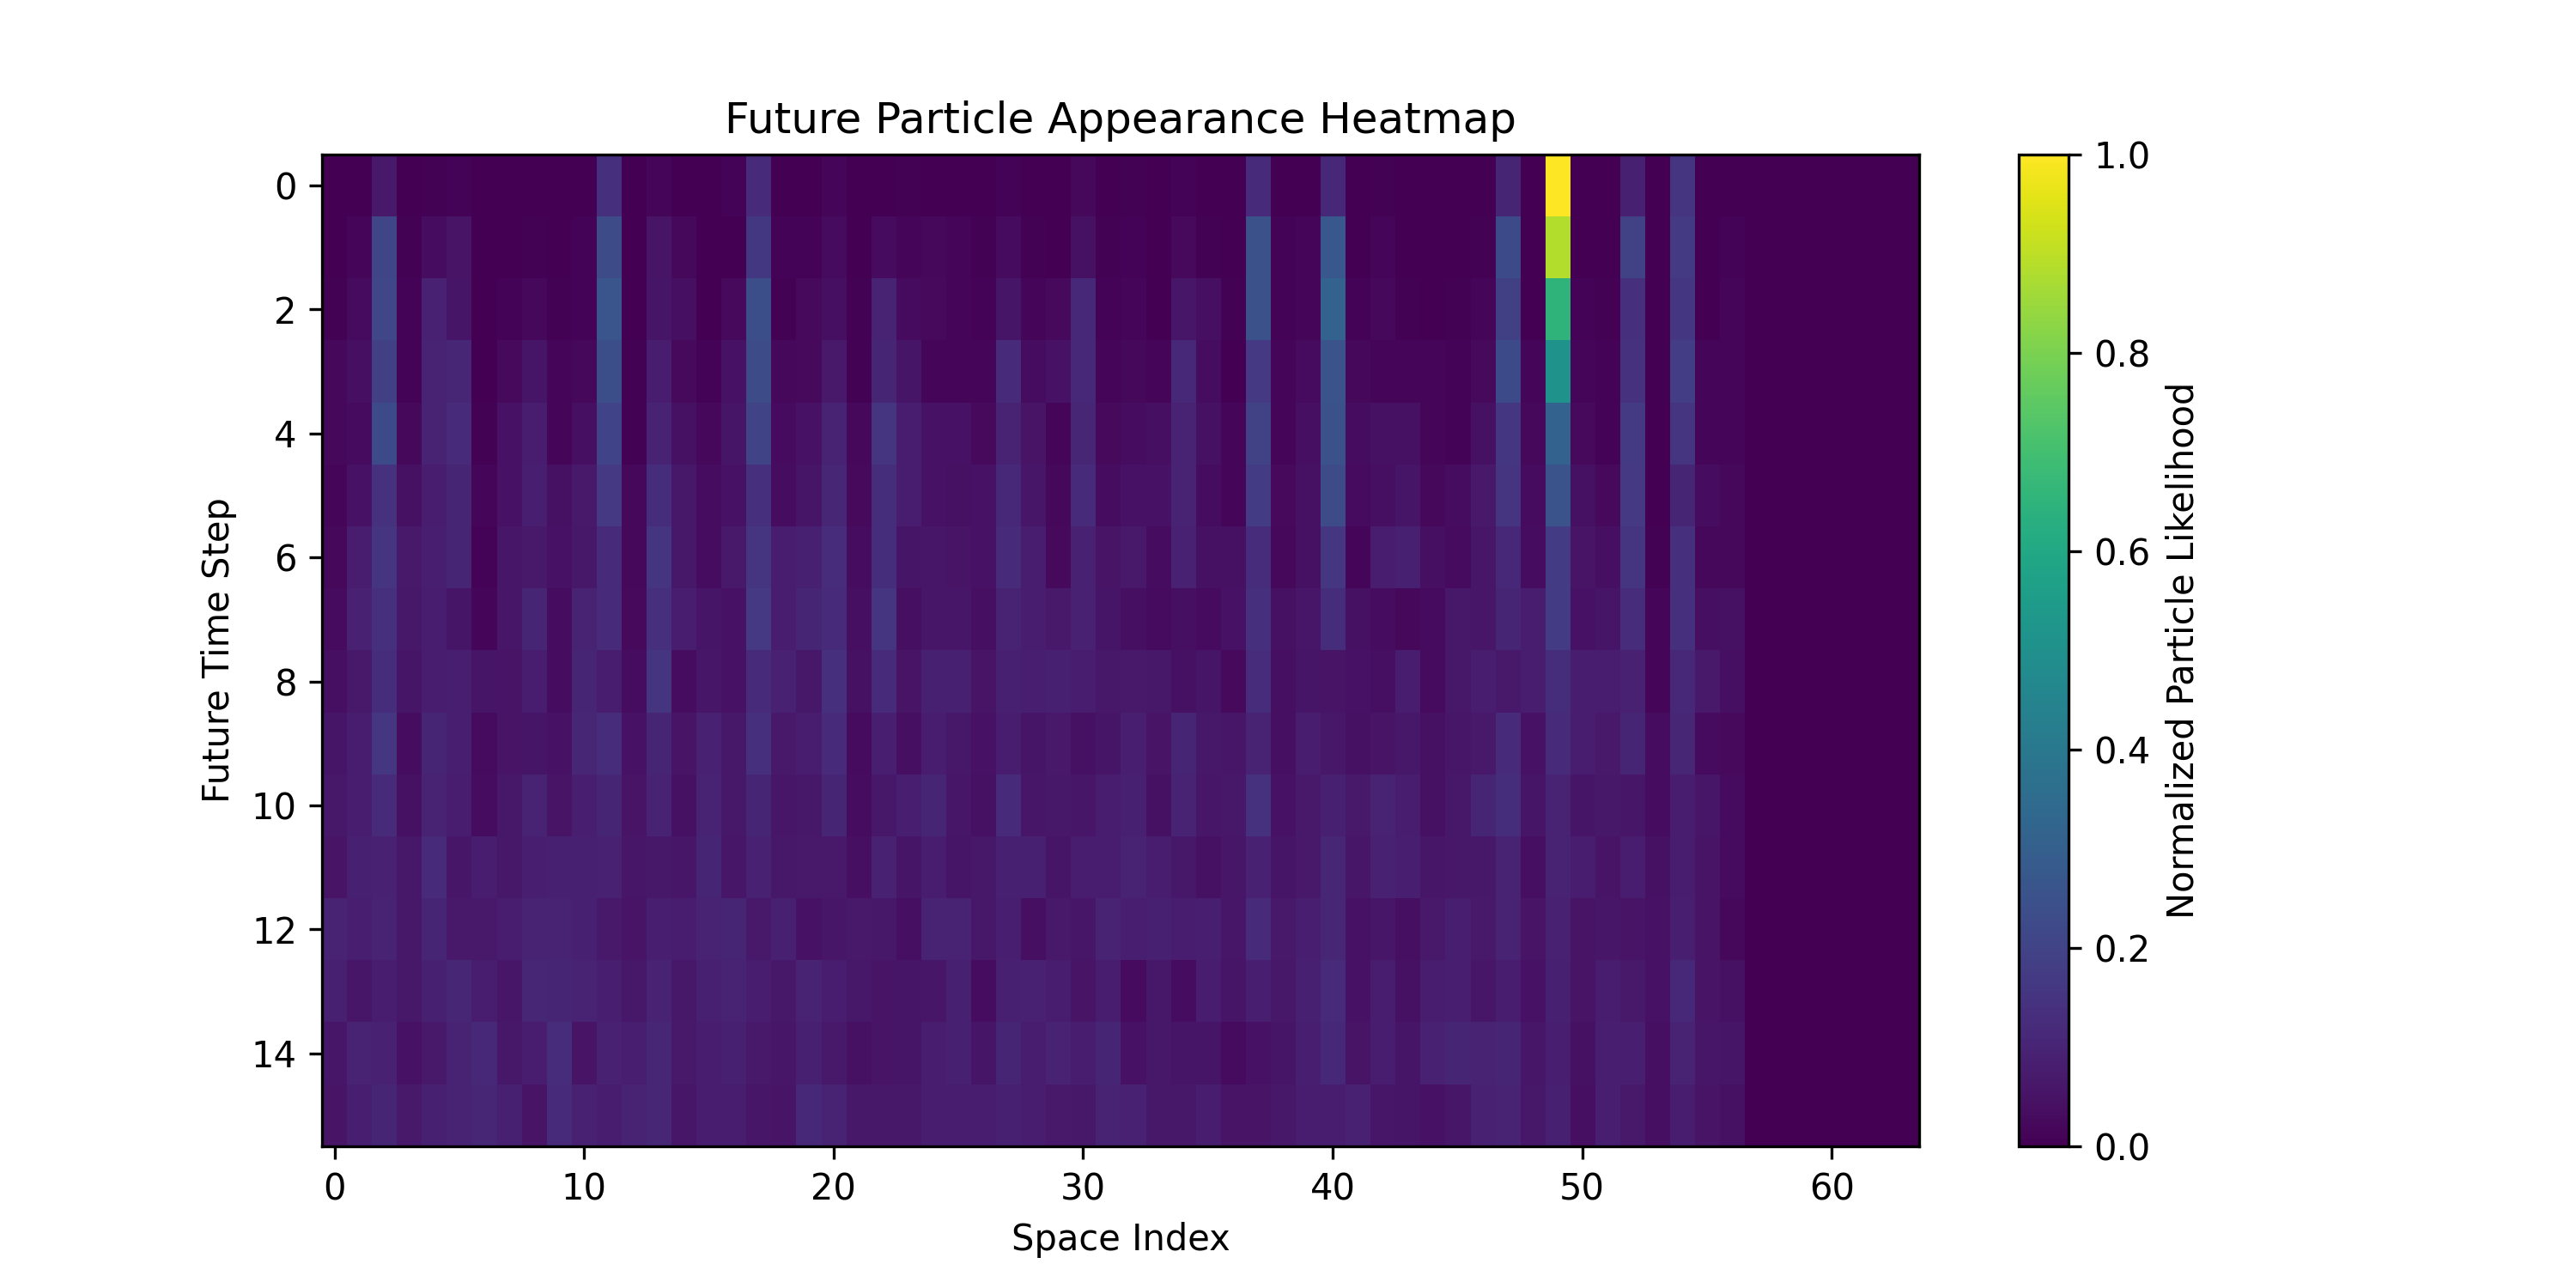
\includegraphics[width=1.0\textwidth]{figures/future_particle_heatmap.png}
    \caption{Heatmap visualizing possible future worlds. The image shows the density of particle trajectories in the future, indicating where observers or particles are likely to find consistent continuations. The future is not a single path but a set of probable continuations shaped by the observer's past. Predictability fades with distance from the current state as possible continuations proliferate.}
    \label{fig:future_particle_heatmap}
\end{figure}

\section{Discussion and Implications}

This model abandons conventional notions of causality and dynamics in favor of a static informational ontology.

Universes are static informational structures, with observer experience arising from statistical compatibility between memory fragments and universe configurations. The “future” corresponds to a distribution over possible continuations, weighted by compression-based likelihood, rather than a uniquely evolving timeline.

There is no fundamental substrate—only bitstrings and the observer's search for consistent continuations. Gravity, time, and quantum effects emerge as statistical preferences under this framework.


\section{Conclusion}

We have proposed a minimal, observer-centric framework in which bitstring universes are filtered by the internal structure of the observer. This model integrates and extends our previous work by showing that classical and quantum phenomena alike can emerge from a single informational substrate, using compression and structural similarity as guiding principles. Probability, persistence, and interference arise not from physical causes but from the combinatorics of observer-compatible paths through the space of possible bitstring universes.

Future work will generalize this framework to support entropic dynamics, relativistic embeddings, and information-theoretic formulations of space, spin, and causality.


\end{document}
